\documentclass{beamer}
\usetheme{Boadilla}

\usepackage{amsmath}
\usepackage{IEEEtrantools}
%\usepackage[caption=false,font=footnotesize]{subfig}
\usepackage{subfig}
\usepackage{animate}
\usepackage{color}

\captionsetup[subfloat]{labelformat=empty}

\title[Variable Rate Tracking]{Dynamical Models for Tracking with the Variable Rate Particle Filter}
\author[P. Bunch \& S. Godsill]{Pete Bunch and Simon Godsill}
\institute[CUED SigProC]{Cambridge University Engineering Department\\ Signal Processing \& Communications Lab}
\date{11th July, 2012}

\begin{document}

\begin{frame}
\titlepage
\end{frame}

\begin{frame}{What's in store...}
\begin{itemize}
  \item What is a variable rate model?
  \item What is a variable rate particle filter?
  \item What dynamical models can we use for tracking with a VRPF?
  \item What's wrong with them?
  \item How can make them better?
  \item Does it work in 3 dimensions?
\end{itemize}
\end{frame}

\begin{frame}
What is a variable rate model?
\end{frame}

\begin{frame}{Conventional Hidden Markov Models for Tracking}
\begin{figure}\centering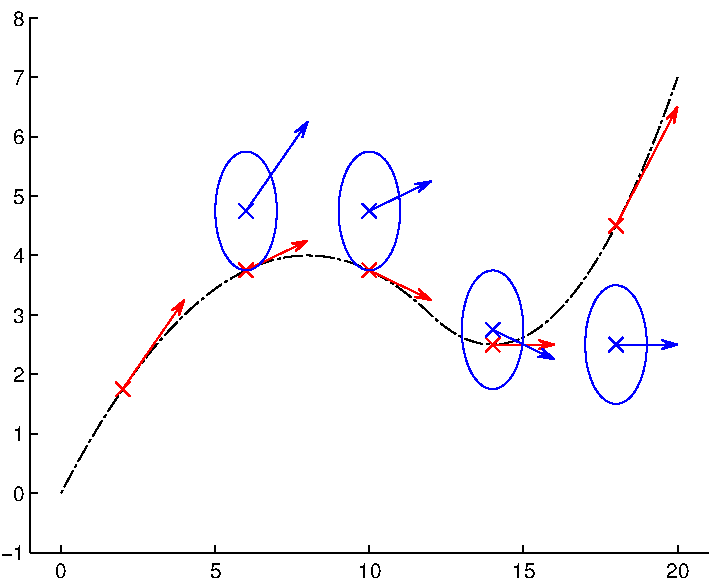
\includegraphics[scale=0.5]{HMM_model.pdf}\end{figure}
\begin{itemize}
  \item Discrete-time
  \item Stochastic Markovian dynamics
  \item Simple
  \item Hard to handle manoeuvres
\end{itemize}
\end{frame}

\begin{frame}{Variable Rate Models for Tracking}
\begin{figure}\centering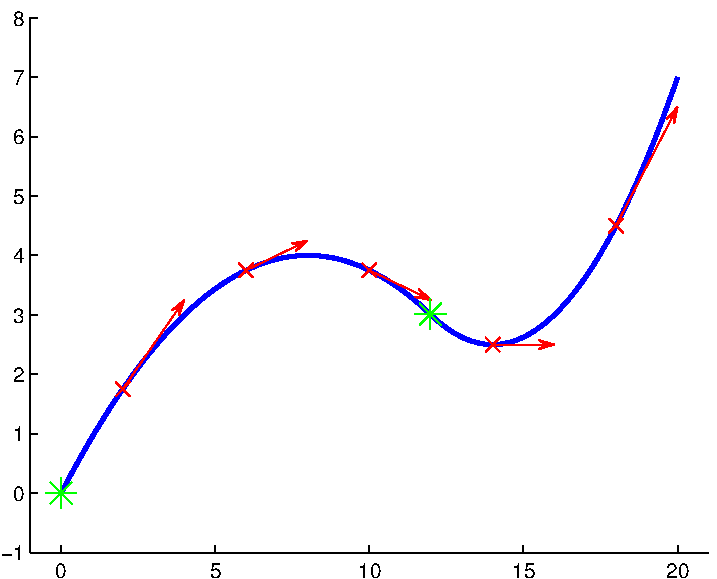
\includegraphics[scale=0.5]{variable_rate_model.pdf}\end{figure}
\begin{itemize}
  \item Continuous-time
  \item Conditionally-deterministic dynamics
  \item Always nonlinear
  \item Handles manoeuvres
\end{itemize}
\end{frame}

\begin{frame}
What is a variable rate particle filter?
\end{frame}

\begin{frame}{The Variable Rate Particle Filter}
\pause Bootstrap particle filter
\begin{itemize}
  \item Proposal: Add a new changepoint or just extend trajectory
  \item Weight update: $w_n \propto w_{n-1} p(y_n|x(t_n))$
\end{itemize}
\pause Improvements
\begin{itemize}
  \item Resample-move
  \item SMC sampler
  \item RJ-MCMC
\end{itemize}
\end{frame}

\begin{frame}
\begin{figure}\animategraphics[poster,width=0.8\textwidth]{100}{animation/vrpf_}{2}{500}\end{figure}
\end{frame}

\begin{frame}
What dynamical models can we use for tracking with a VRPF?
\end{frame}

\begin{frame}{VR Tracking Models I: Cartesian Coordinates}
\begin{IEEEeqnarray*}{rCl}
 \begin{bmatrix} \dot{x}_1(t) \\ \dot{x}_2(t) \\ \ddot{x}_1(t) \\ \ddot{x}_2(t) \end{bmatrix} & = & \begin{bmatrix} 0 & 0 & 1 & 0 \\ 0 & 0 & 0 & 1 \\ 0 & 0 & 0 & 0 \\ 0 & 0 & 0 & 0 \end{bmatrix} \begin{bmatrix} x_1(t) \\ x_2(t) \\ \dot{x}_1(t) \\ \dot{x}_2(t) \end{bmatrix} + \begin{bmatrix} 0 & 0 \\ 0 & 0 \\ 1 & 0 \\ 0 & 1 \end{bmatrix} \begin{bmatrix} a_{1,k} \\ a_{2,k} \end{bmatrix} \\
 & & \\
 & & \tau_k \leq t < \tau_{k+1}
\end{IEEEeqnarray*}
\pause
\begin{IEEEeqnarray*}{rCl}
 \begin{bmatrix} x_1(t) \\ x_2(t) \\ \dot{x}_1(t) \\ \dot{x}_2(t) \end{bmatrix} & = & \begin{bmatrix} 1 & 0 & \Delta t & 0 \\ 0 & 1 & 0 & \Delta t \\ 0 & 0 & 1 & 0 \\ 0 & 0 & 0 & 1 \end{bmatrix} \begin{bmatrix} x_1(\tau_k) \\ x_2(\tau_k) \\ \dot{x}_1(\tau_k) \\ \dot{x}_2(\tau_k) \end{bmatrix} + \begin{bmatrix} \frac{1}{2}\Delta t^2 & 0 \\ 0 & \frac{1}{2}\Delta t^2 \\ \Delta t & 0 \\ 0 & \Delta t \end{bmatrix} \begin{bmatrix} a_{1,k} \\ a_{2,k} \end{bmatrix} \\
 & & \\
 & & \Delta t = t - \tau_k
\end{IEEEeqnarray*}
\end{frame}

\begin{frame}{VR Tracking Models II: Intrinsic Coordinates}
\begin{IEEEeqnarray*}{rCl}
 \dot{s}(t) & = & a_{T,k} \\
 s(t) \dot{\psi}(t) & = & a_{N,k} \\
 \dot{x}_1(t) & = & s(t) \cos(\psi(t)) \\
 \dot{x}_2(t) & = & s(t) \sin(\psi(t)) \\
 & & \\
 & & \tau_k \leq t < \tau_{k+1}
\end{IEEEeqnarray*}
\end{frame}

\begin{frame}
\begin{IEEEeqnarray*}{rCl}
\dot{s}(t) & = & \dot{s}(\tau_k) + a_{T,k} \Delta t \label{eq:2D_ICmodel_start} \\
\psi(t) & = & \psi(\tau_k) + \frac{a_{N,k}}{a_{T,k}} \log \left( \frac{\dot{s}(t)}{\dot{s}(\tau_k)} \right) \\
x(t) & = & x(\tau_k) + \frac{ \dot{s}(t)^2 }{ 4 a_{T,k}^2 + a_{N,k}^2 } \left[  a_{N,k} \sin(\psi(t)) + 2 a_{T,k} \cos(\psi(t))  \right] \\
     &   & - \frac{\dot{s}(\tau_k)^2}{4 a_{T,k}^2 + a_{N,k}^2} \left[  a_{N,k} \sin(\psi(\tau_k)) + 2 a_{T,k} \cos(\psi(\tau_k))  \right] \\
y(t) & = & y(\tau_k) + \frac{ \dot{s}(t)^2 }{ 4 a_{T,k}^2 + a_{N,k}^2 } \left[ -a_{N,k} \cos(\psi(t)) + 2 a_{T,k} \sin(\psi(t))  \right] \\
     &   & - \frac{\dot{s}(\tau_k)^2}{4 a_{T,k}^2 + a_{N,k}^2} \left[  -a_{N,k} \cos(\psi(\tau_k)) + 2 a_{T,k} \sin(\psi(\tau_k))  \right] \\
 & & \\
 & & \Delta t = t - \tau_k
\end{IEEEeqnarray*}
\end{frame}

\begin{frame}
What's wrong with them?
\end{frame}

\begin{frame}{A Problem: Model Deficiency}
\begin{itemize}
  \item 4 state variables governed by 2 motion parameters
  \item From a given state and time, not all future states are achievable
\end{itemize}
Problems:
\begin{itemize}
  \item Poor robustness to model errors
  \item Forward-backward smoothing does not work
\end{itemize}
\end{frame}

\begin{frame}{A Familiar Example}
\begin{IEEEeqnarray*}{rCl}
 x_{n} & = & A x_{n-1} + w_{n} \\
 w_n & \sim & \mathcal{N}(.|0, Q)
\end{IEEEeqnarray*}
\begin{IEEEeqnarray*}{rClrCl}
 Q_1 & = & \sigma^2 \begin{bmatrix} \frac{1}{3}\Delta t^3 & \frac{1}{2}\Delta t^2 \\ \frac{1}{2}\Delta t^2 & \Delta t \\ \end{bmatrix} \qquad & \qquad Q_2 & = & \sigma^2 \begin{bmatrix} \frac{1}{4}\Delta t^3 & \frac{1}{2}\Delta t^2 \\ \frac{1}{2}\Delta t^2 & \Delta t \end{bmatrix}
\end{IEEEeqnarray*}
\begin{figure}
\centering
\subfloat[$Q_1$]{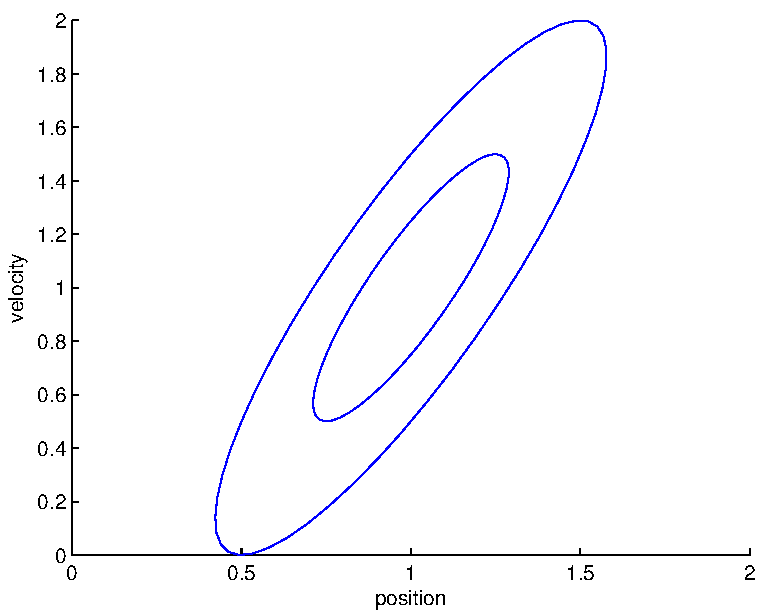
\includegraphics[scale=0.2]{full_rank.pdf}} \qquad \qquad
\subfloat[$Q_2$]{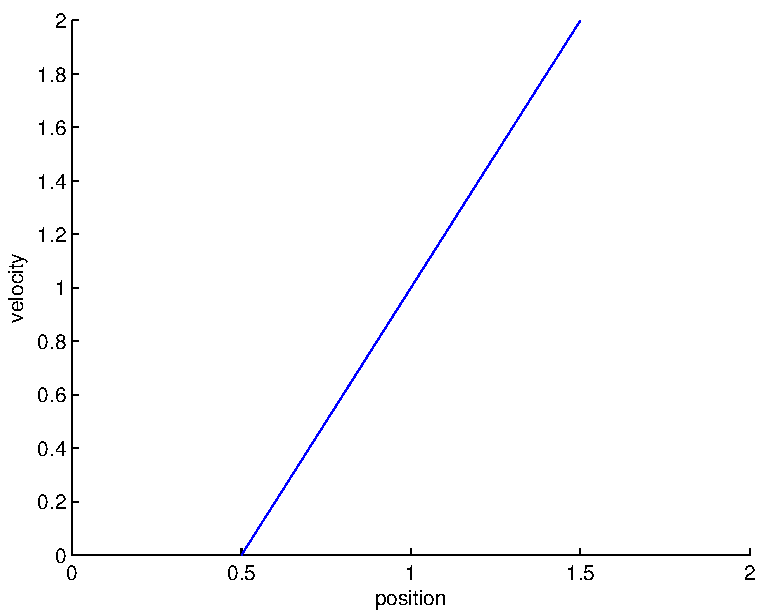
\includegraphics[scale=0.2]{deficient.pdf}}
\end{figure}
\end{frame}

\begin{frame}
How can make them better?
\end{frame}

\begin{frame}{The Solution: Add More Parameters}
\begin{IEEEeqnarray*}{rCl}
 \dot{s}(t) & = & a_{T,k} \\
 s(t) \dot{\psi}(t) & = & a_{N,k} \\
 \dot{x}_1(t) & = & s(t) \cos(\psi(t)) + d_{1,k} \\
 \dot{x}_2(t) & = & s(t) \sin(\psi(t)) + d_{2,k} \\
 & & \\
 & & \tau_k \leq t < \tau_{k+1}
\end{IEEEeqnarray*}
\end{frame}

\begin{frame}{Variable Rate Smoothing}
\begin{figure}
\centering
\subfloat[Filter]{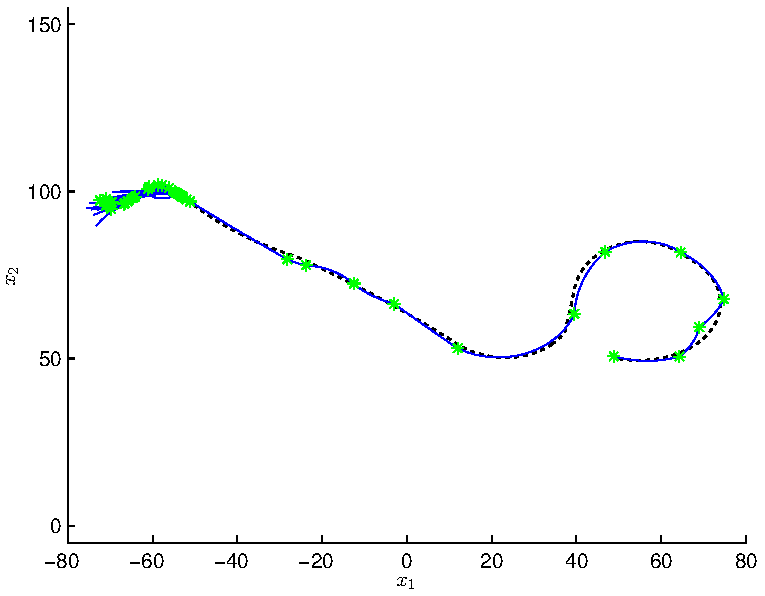
\includegraphics[width=0.4\textwidth]{2Dfilter_big.pdf}} \qquad \qquad
\subfloat[Smoother]{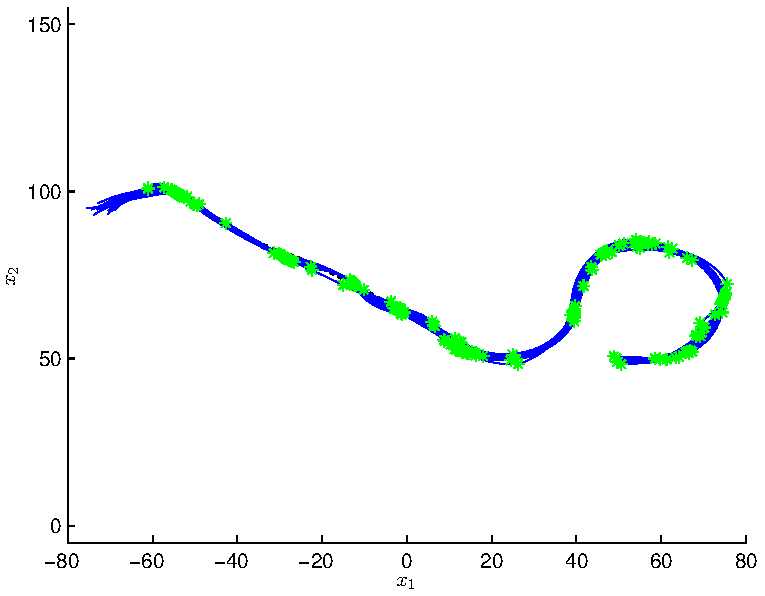
\includegraphics[width=0.4\textwidth]{2Dsmoother_big.pdf}}
\end{figure}
\end{frame}

\begin{frame}
Does it work in 3 dimensions?
\end{frame}

\begin{frame}{3D Intrinsic Coordinate Tracking}
\begin{IEEEeqnarray*}{rCl}
\dot{s}(t)            & = & a_{T,k} \\
\dot{\mathbf{e}}_T(t) & = & \frac{a_{N,k}}{s(t)} \mathbf{e}_N(t) \\
\dot{\mathbf{e}}_N(t) & = & - \frac{a_{N,k}}{s(t)} \mathbf{e}_T(t) \\
\dot{\mathbf{e}}_B(t) & = & \mathbf{0}     .
\end{IEEEeqnarray*}
\end{frame}

\begin{frame}{3D Intrinsic Coordinate Tracking}
\vspace{2em}
{\tiny \color{black}{ \begin{IEEEeqnarray*}{rCl}
\dot{s}(t) &=& \dot{s}(\tau_k) + a_{T,k} \Delta t \\
\begin{bmatrix}\mathbf{e}_T(t)^T \\ \mathbf{e}_N(t)^T \\ \mathbf{e}_B(t)^T \end{bmatrix} &=& \begin{bmatrix}\cos(\Delta \psi(t)) & \sin(\Delta \psi(t)) & 0 \\ -\sin(\Delta \psi(t)) & \cos(\Delta \psi(t)) & 0 \\ 0 & 0 & 1 \end{bmatrix} \begin{bmatrix}\mathbf{e}_{T}(\tau_k)^T \\ \mathbf{e}_{N}(\tau_k)^T \\ \mathbf{e}_{B}(\tau_k)^T \end{bmatrix} \\
\Delta \psi(t) &=& \frac{a_{N,k}}{a_{T,k}} \log \left( \frac{\dot{s}(t)}{\dot{s}(\tau_k)} \right)
\end{IEEEeqnarray*}
\begin{IEEEeqnarray*}{rCl}
\mathbf{v}(t) & = & \dot{s}(t) \mathbf{e}_T(t) \\
\mathbf{r}(t) & = & \mathbf{r}(\tau_k) + \frac{1}{a_{N,k}^2 + 4 a_{T,k}^2} \times \begin{bmatrix} \mathbf{e}_{T}(\tau_k) & \mathbf{e}_{N}(\tau_k) \end{bmatrix} \begin{bmatrix} \zeta_{1}(t) & \zeta_{2}(t) \\ \zeta_{2}(t) & -\zeta_{1}(t) \end{bmatrix}  \begin{bmatrix} 2 a_{T,k} \\ a_{N,k} \end{bmatrix} \nonumber \\
\zeta_{1}(t)  & = & \cos(\Delta \psi(t)) \dot{s}(t)^2 - \dot{s}(\tau_k)^2 \\
\zeta_{1}(t)  & = & \sin(\Delta \psi(t)) \dot{s}(t)^2
\end{IEEEeqnarray*} }}
\end{frame}

\begin{frame}{3D Intrinsic Coordinate Tracking}
\begin{figure}
\centering
\subfloat[Cartesian]{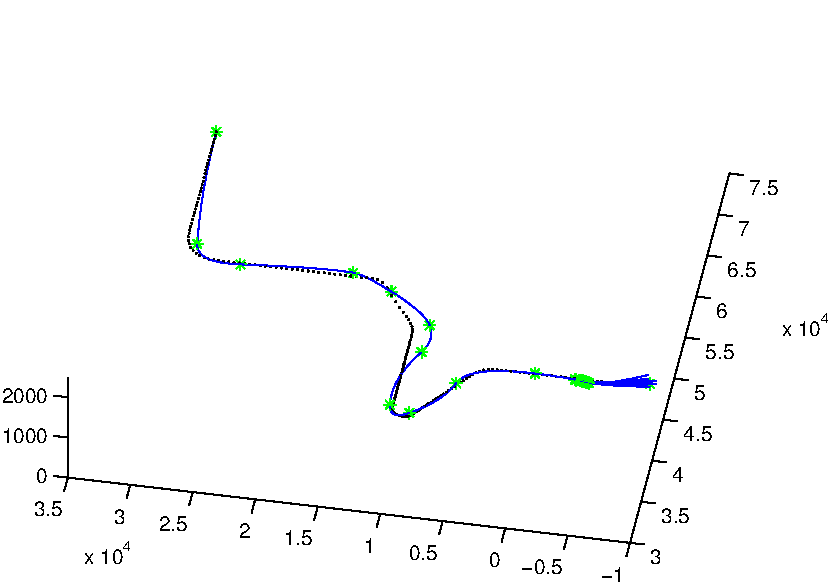
\includegraphics[width=0.4\textwidth]{3DCartesian_big.pdf}} \qquad \qquad
\subfloat[Intrinsic]{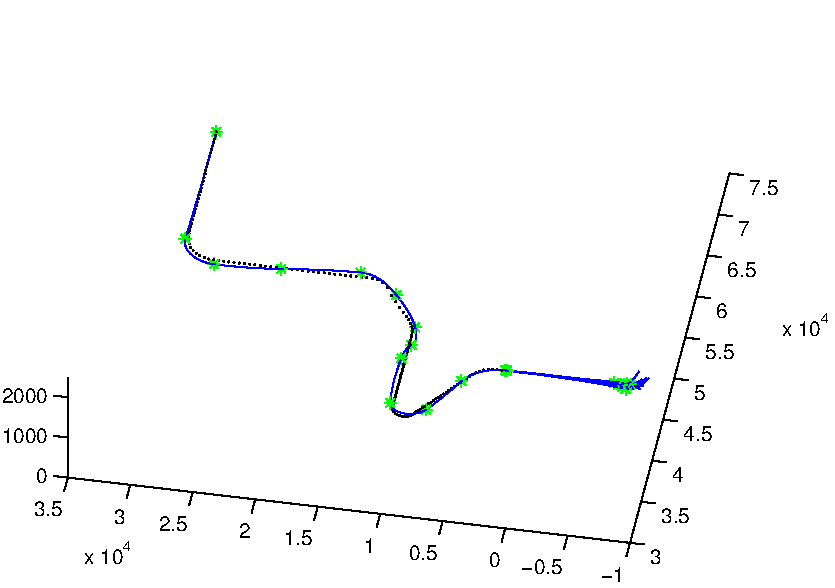
\includegraphics[width=0.4\textwidth]{3DIntrinsic_big.pdf}}
\end{figure}
\end{frame}

\begin{frame}{Summary}
\begin{itemize}
  \item Variable rate framework elegantly handles manoeuvres, changepoints and model-switching.
  \item Variable rate particle filter may be used for inference in this framework.
  \item Basic VR tracking models are uncontrollable - thwarts smoothing algorithms.
  \item New augmented model improves estimation and may be used for smoothing.
  \item Intrinsic coordinate model has been extended to work in 3D - piecewise planar assumption.
\end{itemize}
\end{frame}

\begin{frame}
\end{frame}

\end{document} 